\documentclass{article}

\usepackage{graphicx}
\usepackage{amsmath}
\usepackage{xepersian}

\settextfont{Times New Roman}

\title{تمرین دوم طراحی سیستم‌های دیجیتال}
\author{پارسا محمدیان -- 98102284}

\begin{document}
\maketitle
\newpage

\section{توضیحات تمرین}
در این تمرین ابتدا 
\lr{ASM}
تقسیم‌کننده خواسته شده رسم کردم. این 
\lr{ASM}
در فایل 
\lr{ASM.vsdx}
موجود است و در شکل 
\ref{asm}
مشاهده می‌شود.

\begin{figure}[!htbp]
    \centering
    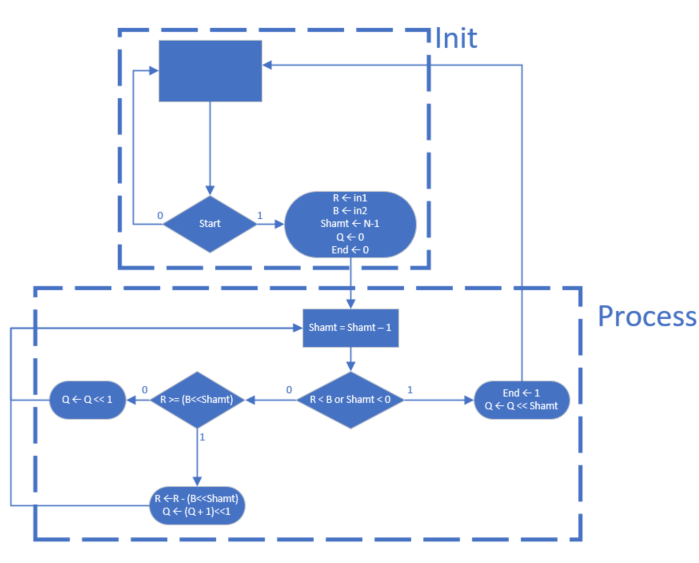
\includegraphics[width=\linewidth]{ASM.png}
    \label{asm}
    \caption{\lr{ASM} تقسیم‌کننده}
\end{figure}

سپس کد وریلاگ هر یک از دو بخش واحد کنترل و مسیر داده را به ترتیب در فایل‌های 
\lr{cu.v}
و
\lr{dp.v}
می‌نویسیم. این دو بخش را در ماژول موجود در فایل 
\lr{subtractor.v}
به یکدیگر متصل می‌کنیم. تست بنچ نیز در فایل 
\lr{tb\_subtractor.v} 
موجود می‌باشد. 

\section{تست مدار}
برای تست مدار 3 بار ورودی مختلف داده‌ایم. شکل موج در شکل 
\ref{tb}
موجود است.

\begin{gather*}
    15 = 7 \times 2 + 1 \\
    40 = 3 \times 13 + 1 \\
    40 = 5 \times 8 + 0
\end{gather*}

\begin{figure}[!htbp]
    \centering
    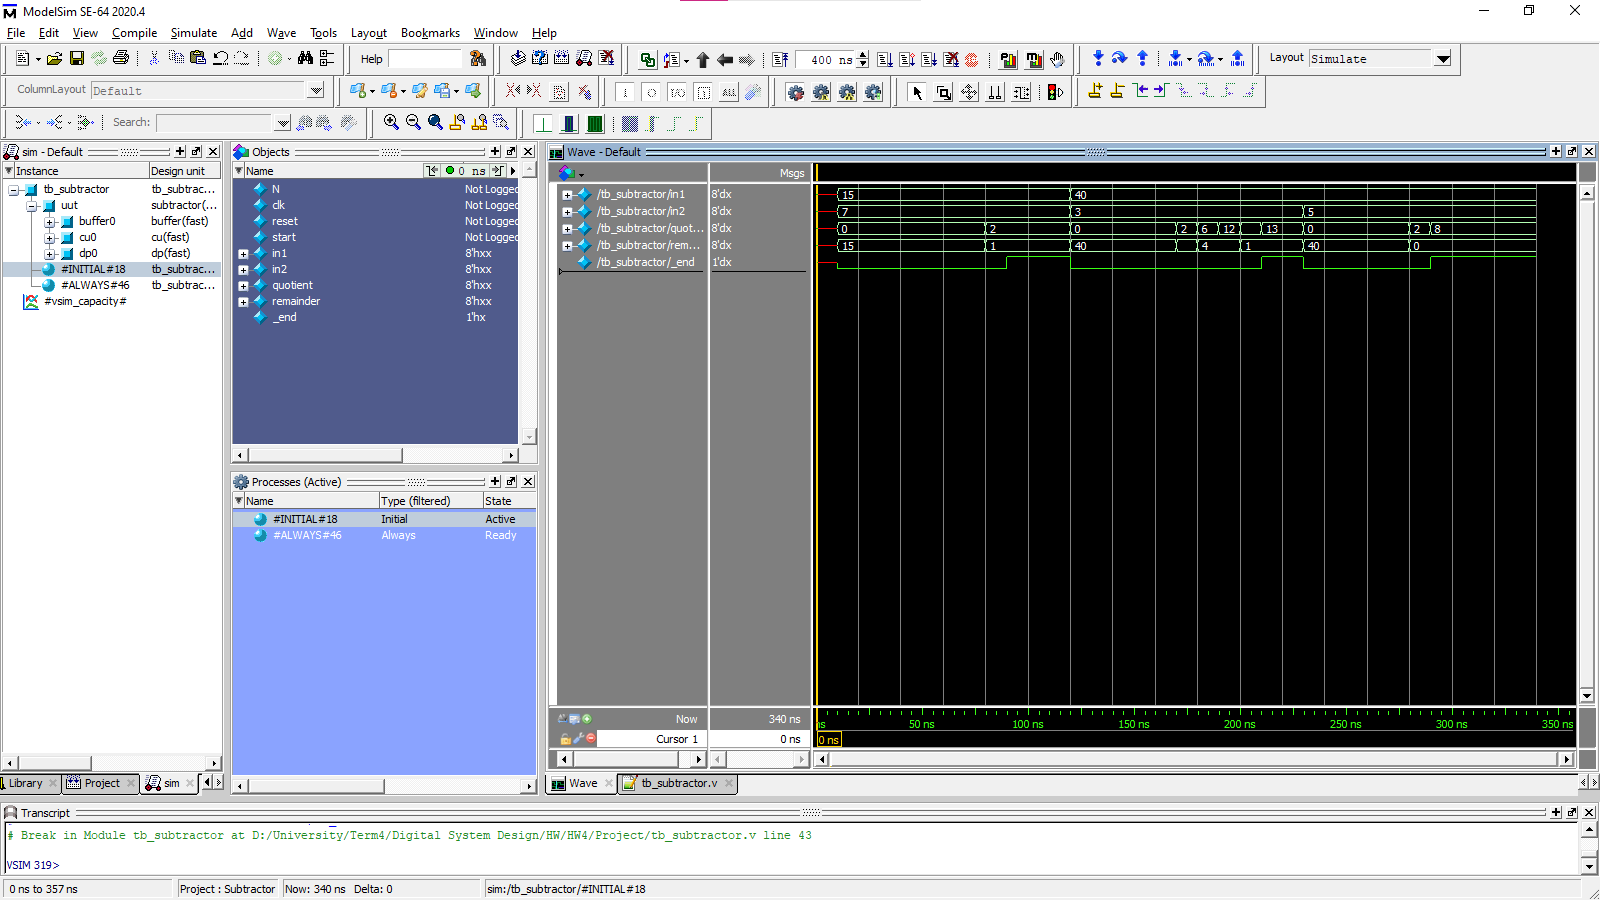
\includegraphics[width=\linewidth]{ModelSim.png}
    \label{tb}
    \caption{تست مدار تقسیم‌کننده}
\end{figure}

\end{document}
